\documentclass[
	% -- opções da classe memoir --
	12pt,				% tamanho da fonte
	openright,			% capítulos começam em pág ímpar (insere página vazia caso preciso)
	oneside,			% para impressão em recto e verso. Oposto a oneside
	a4paper,			% tamanho do papel. 
	% -- opções da classe abntex2 --
	chapter=TITLE,		% títulos de capítulos convertidos em letras maiúsculas
	%section=TITLE,		% títulos de seções convertidos em letras maiúsculas
	%subsection=TITLE,	% títulos de subseções convertidos em letras maiúsculas
	%subsubsection=TITLE,% títulos de subsubseções convertidos em letras maiúsculas
	% -- opções do pacote babel --
	english,			% idioma adicional para hifenização
	%french,				% idioma adicional para hifenização
	%spanish,			% idioma adicional para hifenização
	brazil				% o último idioma é o principal do documento
	]{abntex2}

    
% ---
% Pacotes básicos 
% ---

%\usepackage{lmodern}			% Usa a fonte Latin Modern
\usepackage{tgtermes}
\usepackage[T1]{fontenc}		% Selecao de codigos de fonte.
\usepackage[utf8]{inputenc}		% Codificacao do documento (conversão automática dos acentos)

\usepackage{color}				% Controle das cores
\usepackage{graphicx}			% Inclusão de gráficos
\usepackage{microtype} 			% para melhorias de justificação
\usepackage{multirow}           %Utilizado para as tabelas
\usepackage[table,xcdraw]{xcolor}%Utilizado para as tabelas 
\usepackage{listings}           %Utilizado para as listas
\usepackage{subfig}             %Utilizado para as legendas
% \usepackage[portuguese,ruled,linesnumbered,lined]{algorithm2e}                           %Utilizado para os algoritmos
% \usepackage{algorithmic}        %Utilizado para os algoritmos
\usepackage{verbatim}
\usepackage{pdfpages}           %Utilizado para criar a capa
\usepackage{pdflscape}
\usepackage{longtable}
\usepackage{float}
\usepackage{adjustbox}


\usepackage{listings}
\usepackage{graphicx}
\usepackage{amssymb}
\usepackage{hyperref}
\usepackage{amssymb}
\usepackage{pifont}

\usepackage[alf,abnt-etal-cite=2]{abntex2cite}	

\def\myversion{2.0 }
\date{}

\newcommand{\thedepartment}{IMC - Instituto de Matemática e Computação}
\newcommand{\thecourse}{Curso de Ciência da Computação}
\newcommand{\thetitle}{Smart Ovitraps}
\newcommand{\thesubtitle}{A Cloud IoT-Ovitrap System}
\newcommand{\theproftitle}{Bacharel em Ciência da Computação}
\newcommand{\thestudent}{Daniel Pinheiro dos Reis}
\newcommand{\theadvisor}{Prof. Dr. Adler Diniz de Souza}
\newcommand{\thecoadvisor}{Profa. Dra. Elisa Rodrigues}
\newcommand{\thecity}{Itajubá}

% ---
% Informações de dados para CAPA e FOLHA DE ROSTO
% ---

\begin{document}

\begin{center}
    \newcommand*{\themonth}{\ifthenelse{\the\month < 2}{Janeiro }
                  {\ifthenelse{\the\month < 3}{Fevereiro }
                  {\ifthenelse{\the\month < 4}{Março }
                  {\ifthenelse{\the\month < 5}{Abril }
                  {\ifthenelse{\the\month < 6}{Maio }
                  {\ifthenelse{\the\month < 7}{Junho }
                  {\ifthenelse{\the\month < 8}{Julho }
                  {\ifthenelse{\the\month < 9}{Agosto }
                  {\ifthenelse{\the\month < 10}{Setembro }
                  {\ifthenelse{\the\month < 11}{Outubro }
                  {\ifthenelse{\the\month < 12}{Novembro }{Dezembro }}}}}}}}}}}}
                  


\begin{center}



  \begin{figure}[hbt!]
		\begin{center}
		   \includegraphics[width=2.8cm]{./imagens/logo_unifei.png}
		\end{center}
	\end{figure}
% 	\vspace{-4cm}

  \Large{\textbf{Universidade Federal de Itajubá}}\\
  \large{\thedepartment}\\
  \large{\thecourse}\\



{ \huge \bfseries \LARGE{\thetitle} \\ [1.0cm]
\emph{\large{\thesubtitle}}
}\\[0.4cm] % Title of your document




  

  \large{\thestudent}\\
  Orientador: \theadvisor\\
  Co-Orientadora: \thecoadvisor\\

\pagenumbering{gobble}

  \par\vfill
  \thecity, \themonth / \the\year

\end{center}

\end{center}

\preambulo{Monografia apresentada como trabalho final de graduação, requisito parcial para a obtenção do título de Bacharel em 
Ciência da Computação, sob orientação da Prof. Dr. Adler Diniz de Souza}
% ---


% ---
% Configurações de aparência do PDF final

% alterando o aspecto da cor azul
\definecolor{blue}{RGB}{0,0,0}

% informações do PDF
\makeatletter
\hypersetup{
 %pagebackref=true,
    pdftitle={\@title}, 
    pdfauthor={\@author},
    pdfsubject={\imprimirpreambulo},
    pdfcreator={LaTeX with abnTeX2},
    pdfkeywords={abnt}{latex}{abntex}{abntex2}{trabalho acadêmico}, 
    linkcolor=black,          	% color of internal links
    citecolor=black,        		% color of links to bibliography
    filecolor=magenta,      		% color of file links
    urlcolor=blue,
    bookmarksdepth=4		
}
\makeatother
% --- 

% ---
% Posiciona figuras e tabelas no topo da página quando adicionadas sozinhas
% em um página em branco. Ver https://github.com/abntex/abntex2/issues/170
\makeatletter
\setlength{\@fptop}{5pt} % Set distance from top of page to first float
\makeatother
% ---

% configurações para atender às regras da ABNT
\setfloatadjustment{quadro}{\centering}
\renewcommand{\ABNTEXchapterfont}{\rmfamily\small\bfseries}
\renewcommand{\ABNTEXchapterfontsize}{\small}
\renewcommand{\ABNTEXsectionfontsize}{\small}
\renewcommand{\ABNTEXsubsectionfontsize}{\small}


\setfloatlocations{quadro}{hbtp} % Ver https://github.com/abntex/abntex2/issues/176
 

% Recuo dos parágrafos
\setlength{\parindent}{0cm}
% Controle do espaçamento entre um capitulo e um parágrafo.
\setlength\afterchapskip{\lineskip}
 % Controle do espaçamento entre um capitulo e um parágrafos tente também \onelineskip
\setlength{\parskip}{0.2cm} 

\pagenumbering{roman}
% Seleciona o idioma do documento (conforme pacotes do babel)
%\selectlanguage{english}
\selectlanguage{brazil}

% Retira espaço extra obsoleto entre as frases.
\frenchspacing 

\newpage
\begin{epigrafe}
    \vspace*{\fill}
	\begin{flushright}
		\textit{"O insucesso é apenas uma oportunidade para recomeçar com mais inteligência"\\
		(Henry Ford)}
	\end{flushright}
\end{epigrafe}

% ---
% Agradecimentos
% ---

\begin{agradecimentos}
Agradeço aos meus pais, por me darem a oportunidade do estudo, à todos os meus professores e amigos por partilharem o conhecimento 
comigo e por poder estar concluindo esse ciclo.

\end{agradecimentos}
% ---

% ---

% ---

% ---
% RESUMOS
% ---

% resumo em português
\setlength{\absparsep}{18pt} % ajusta o espaçamento dos parágrafos do resumo

\begin{resumo}

A intensificação dos arbovírus (dengue, zika, chikungunya, etc) destaca a necessidade de um controle eficaz do seu vetor de transmissão, 
o mosquito Aedes. Para isso, foram criadas as Ovitraps, armadilhas que capturam os ovos depositados pelas fêmeas impedindo a multiplicação 
da população de mosquitos. Apesar dos vários modelos de Ovitraps existentes poucos, ou quase nenhum deles, aplicam algum conceito de tecnologia
 em seu desenvolvimento, tais modelos necessitam de um profissional que realize o trabalho de campo de coleta das armadilhas e de um 
 profissional para análise dos dados coletados. Este trabalho busca desenvolver uma ovitrap que facilite o trabalho de campo de coleta 
 e de analise dos dados. Aplicando modelos de IoT no desenvolvimento de uma ovitrap "inteligente" capaz de capturar os dados e 
 disponibiliza-los na nuvem para que possam ser acessados de maneira remota em qualquer lugar com acesso a internet.

\textbf{Palavras-chave}:  Armadilha, Ovitrap, IoT, Dengue, Zika e Chikungunya.

\end{resumo}

% resumo em inglês
\begin{resumo}[Abstract]
\begin{otherlanguage*}{english}

The intensification of arboviroses (dengue, zika, chikungunya, etc.) highlights the need for effective control of its transmission vector, 
the female Aedes mosquito. For this purpose, Ovitrap were created, traps that capture the eggs deposited by the females, preventing the 
multiplication of the mosquito population. Despite the several existing Ovitraps models, few or almost none of them apply any concept of 
technology in their development, such models need a professional to carry out the fieldwork to collect the traps and a professional to 
analyze the collected data. This work seeks to develop a platform that facilitates the field work of collecting and analyzing data. For 
this, IoT models are applied in the development of a "smart" device capable of capturing data and making it available in the cloud so that 
it can be accessed remotely anywhere with Internet access.

\textbf{Palavras-chave}: Traps, Ovitrap, IoT, Dengue, Zika and Chikungunya.

\end{otherlanguage*}
\end{resumo}

% ---

% ---
% inserir lista de ilustrações
% ---
\pdfbookmark[0]{\listfigurename}{lof}
\listoffigures*
\cleardoublepage
% ---

% ---
% inserir lista de tabelas
% ---
\pdfbookmark[0]{\listtablename}{lot}
\listoftables*
\cleardoublepage
% ---

% ---
% inserir lista de abreviaturas e siglas
% ---
\begin{siglas}
  \item[IoT] Internet of Things
  \item[HTTP] HyperText Transfer Protocol
  \item[AWS] Amazon Web Services
  \item[S3] Amazon Simple Storage Service
  \item[EC2] Amazon Elastic Compute Cloud
  \item[MUI] Material-UI 
Artificiais 
\end{siglas}

% ---
% inserir o sumario
% ---
\pdfbookmark[0]{\contentsname}{toc}
\tableofcontents*
\cleardoublepage
% ---



% ----------------------------------------------------------
% ELEMENTOS TEXTUAIS
% ----------------------------------------------------------
\textual

\pagenumbering{arabic}
\setcounter{page}{12}

\chapter{Introdução}
A intensificação dos arbovírus (dengue, zika, chikungunya etc) destaca a necessidade de
um controle eficaz do seu vetor de transmissão, o mosquito Aedes. A principal
medida de prevenção dos arbovírus é o controle da população do mosquito. A
implementação de medidas preventivas requer ferramentas de vigilância eficientes que
permitam prever a população real de mosquitos \cite{ISMALIZA2019}. Uma ferramenta de controle que vem
sendo utilizada desde a década de 70 são as ovitraps \cite{LOK1977}

\section{O que é uma ovitrap?}

Ovitraps são armadilhas desenvolvidas para capturar larvas e ou mosquitos. A primeira ovitrap que se tem informação (Figura 1) é creditada a 
Loki 1977 \cite{LOK1977}. A ovitrap de Loki consiste de um recipiente cilíndrico preto, cheio de água,
com uma abertura de malha trançada no topo, com duas pás de madeira sob ela. Embora a
fêmea do mosquito que deposita seus ovos na armadilha não seja morta, os filhotes que
eclodem dos ovos ficam presos pela malha trançada e morrem afogados.

\begin{figure}[h!]
\centering
\includegraphics[scale=1.6]{imagens/ovitrapLoki.jpg}
\caption{Primeiro modelo de ovitrap, desenvolvido na década de 70}
    \label{fig:OvitrapLoki}
    \legend{Disponível em: \nolinkurl{https://www.appropedia.org/Ovitrap}. Acesso em: \today}
\end{figure}

\section{Evolução das ovitraps}

Na evolução das ovitraps foram criadas ovitraps letais, no sentido de, capturar e matar o mosquito fêmea. A primeira delas utilizava uma fita
tratada com inseticida, nas paredes do seu interior, que matava as fêmeas atraídas pela
água, porém foi observado que o mosquito ganhava resistência ao inseticida ao longo do
tempo \cite{BRIANJJOHNSON2017}. Depois foi desenvolvido um modelo que ao invés de uma fita com inseticida
utilizava uma fita adesiva que capturava a fêmea do mosquito \cite{BRIANJJOHNSON2017}. Apesar de eficientes e 
baratas, as ovitraps até então, eram pequenas, o que além de exigir manutenção em curtos
períodos de tempo, não eram tão atrativas as fêmeas do mosquito \cite{BRIANJJOHNSON2017}. Foi desenvolvido
então, modelos maiores, mais atrativos às fêmeas do mosquito e que demandavam
manutenções em períodos de tempo maiores.

\begin{figure}[h!]
\centering
\includegraphics[scale=0.3]{imagens/exemplosovitraps.png}
 \caption{(A) Standard Lethal Ovitrap (LO), (B) National Environmental Agency Singapore Sticky Ovitrap (SO), (C) MosquiTRAP 
 Sticky Ovitrap (SO), (D) Biogents Gravid Aedes Trap (GAT), (E) Centers for Disease Control (CDC) Autocidal Gravid Ovitrap(AGO)}
    \label{fig:evolucaoOvitraps}
    \legend{Disponível em: \nolinkurl{https://www.researchgate.net/publication/312158747_The_State_of_the_Art_of_Lethal_Oviposition_Trap-Based_Mass_Interventions_for_Arboviral_Control/figures}. Acesso em: \today}
\end{figure}

Embora as armadilhas sejam diferentes no design, tanto o AGO (E) quanto o GAT (D)
alcançaram o efeito desejado superando as ovitraps padrão em atratividade para o Aedes.
Estudos em Porto Rico demonstraram que a AGO capturou mais fêmeas grávidas e
forneceu maior sensibilidade do que as ovitraps convencionais \cite{BRIANJJOHNSON2017}, enquanto em testes no norte da 
Austrália, os GATs coletaram de 2 a 4 vezes mais Aedes fêmeas que
duas variações de ovitraps, o MosquiTRAP e o ovitrap pegajoso duplo. 

\section{Motivação}
Apesar da variação de modelos, todos eles precisam de um agente que faça o trabalho de
campo de coletar os dados e prestar manutenção nas armadilhas. Em uma pesquisa
bibliográfica encontrou-se apenas um modelo que emprega o conceito de IoT em ovitrap, o modelo desenvolvido por Ismaliza e outros \cite{ISMALIZA2019} (Figura 3)

\begin{figure}[H]
\centering
\includegraphics[scale=0.4]{imagens/smartovitrap.png}
\includegraphics[scale=0.5]{imagens/smartovitrap2.png}
 \caption{Modelo de ovitrap desenvolvido por Ismaliza Isa et al. }
    \label{fig:ovitrapIsmaliza}
    \legend{Disponível em: \nolinkurl{https://www.researchgate.net/publication/337160411_An_IoT-Based_Ovitrap_System_Applied_for_Aedes_Mosquito_Surveillance/figures}. Acesso em: \today}
\end{figure}

O modelo desenvolvido por Ismaliza e outros é uma ovitrap sticker,
além de capturar o mosquito, a armadilha possui um sensor (VL53L0X) em seu interior que conta a
quantidade de mosquitos que passaram pela armadilha, sendo eles capturados, ou não, por
ela. Este número é mostrado no display da armadilha e enviado para uma aplicação web
que pode ser acessada através de um navegador em qualquer dispositivo conectado a
internet.

Diante do exposto, este trabalho busca desenvolver uma solução para o controle da
população do mosquito Aedes, que seja mais rápida e eficaz que o método tradicional de
controle, utilizando para isso recursos de tecnologia.

\section{Justificativa}

O método tradicional de controle exige trabalho de campo para coletar e analisar os dados
das ovitraps. Este trabalho geralmente é feito por um ou mais agentes que vão até o local
da armadilha para coletar os ovos e mosquitos para análises futuras. Tomando como
exemplo um cenário com mais de 100 armadilhas, o trabalho de coleta de todas as
armadilhas consumiria um tempo de deslocamento do agente proporcional ao número de
armadilhas. Este tempo poderia ser reduzido utilizando a solução proposta por esse trabalho, em que a quantidade capturada de mosquitos,
bem como a localização de cada armadilha é mostrada em um mapa, facilitando a análise e posterior tomada de decisão.

\chapter{Desenvolvimento}

\section{A ideia inicial}

A princípio a ideia inicial deste trabalho era desenvolver uma armadilha que pudesse além de capturar, também fotografar os mosquitos, para depois aplicar processamento digital de 
imagens e catalogar as espécies de mosquitos fotografadas. E se não bastasse isso, também havia uma câmera submersa na água da armadilha para que fosse possível 
fotografar as larvas do mosquito.

\begin{figure}[H]
    \centering
    \includegraphics[scale=0.09, angle=-90]{imagens/IMG_8989.jpg}
    \caption{Primeiros testes}
        \label{fig:aprincipio}
        \legend{FONTE: Autor}
    \end{figure}

A figura acima é primeira foto do desenvolvimento deste trabalho, ela mostra um módulo NodeMCU, um sensor laser (o mesmo usado no protótipo final), 
um sensor ultrassônico, um módulo ESP32-CAM e uma câmera GoPro. A foto foi tirada no primeiro de vários testes. 

O primeiro teste consistia em ter duas câmeras, uma para fotografar 
os mosquitos (ESP32-CAM), e uma para as larvas (GoPro). A câmera GoPro possui um web server integrado, onde é possível via requisições HTTP, tirar fotos, gravar vídeos e controlar 
várias outras funções da câmera, o ESP32-CAM também possui wi-fi integrado. Então, neste primeiro modelo, a câmera esp era ativada pelo sensor laser, e a GoPro era ativada a cada 1 hora, 
lembre-se que a GoPro ficaria submersa e seria responsável por fotografar o desenvolvimento das larvas do mosquito. 
Uma das dificuldades encontradas neste primeiro modelo, era que além de se conectar com o web server da GoPro, 
o modulo ESP32-CAM também se conectava com uma rede Wifi externa, através da qual enviava as fotos via requisição HTTP para API. 
O tempo de envio das fotos da GoPro para API era um pouco lento, devido a alta resolução das fotos, já o tempo do ESP32 era aceitável. 
Outro ponto era que essas fotos ficavam armazenadas em um cartão Micro-SD no módulo ESP32-CAM. O fato de ter que conectar em duas redes diferentes, 
ter de usar um cartão Micro-SD, além do custo do projeto ficar elevado devido a GoPro, foi desenvolvido um segundo teste sem a GoPro, apenas 
com o ESP32-CAM e o sensor laser.

\begin{figure}[H]
    \centering
    \includegraphics[scale=0.2]{imagens/larvasMosquitos.png}
    \caption{Esquema de pastas de fotos para larvas e mosquitos no Amazon S3}
        \label{fig:larvasMosquitos}
        \legend{FONTE: Autor}
    \end{figure}

Neste segundo teste havia apenas uma câmera ESP32-CAM, utilizando um cartão Micro-SD e fixada no teto da armadilha, o fato de usar apenas uma câmera, eliminou a necessidade 
de se conectar em duas redes diferentes, e o tempo de upload de arquivos para API era menor que do primeiro teste, uma vez que as fotos tiradas pelo ESP32-CAM
tem no máximo 2MB de resolução. Se por um lado isso é bom para comunicação com a API, por outro lado é ruim, pois é praticamente impossível detectar um mosquito na foto registrada, 
fator esse que levou a um terceiro teste que deu origem ao protótipo apresentado a seguir.

\begin{figure}[H]
    \centering
    \includegraphics[scale=0.1]{imagens/fotoESP32.jpeg}
    \caption{Foto registrada pelo ESP32-CAM}
        \label{fig:fotoesp32}
        \legend{FONTE: Autor}
    \end{figure}

Nesta seção busca-se descrever as etapas de desenvolvimento da solução proposta. O desenvolvimento se dividiu em três frentes:

\begin{itemize}
    \item Ovitrap:
        \begin{itemize}
        \item Desenvolver uma ovitrap que atraía e capture mosquitos fêmea.
        \end{itemize}
    \item Hardware:
        \begin{itemize}
        \item Contar quantos mosquitos passaram pela armadilha.
        \item Enviar dados coletados da armadilha de maneira segura para uma API.
        \end{itemize}
    \item Software:
        \begin{itemize}
        \item Desenvolver uma API para receber dados de múltiplas armadilhas, tratá-los e armazená-los de maneira segura em um 
        banco de dados.
        \item Disponibilizar os dados armazenados para que sejam consumidos por outras aplicações.
        \item Desenvolver uma aplicação web para consumir os dados fornecidos pela API.
        \end{itemize}
\end{itemize}

\section{Ovitrap}
Um dos grandes desafios ao se desenvolver uma ovitrap é torná-la atraente para as fêmeas do mosquito, isto é, fazer com que a fêmea 
do mosquito deposite seus ovos na ovitrap 
e não em outro lugar próximo a ela. Testes feitos por \cite{DAVIDF2011} e \cite{VALERIE2016} constataram que os mosquitos fêmeas 
são atraídos por ovitraps totalmente pretas.

\begin{figure}[H]
\centering
\includegraphics[scale=0.7]{imagens/tileshop.jpeg}
\caption{Padrões em ovitraps}
    \legend{Disponível em: \nolinkurl{https://www.ncbi.nlm.nih.gov/pmc/articles/PMC4988764/figure/pone.0160386.g009/}. Acesso em: \today}
\end{figure}

Outro ponto relevante ao se projetar uma ovitrap é o seu tamanho, segundo \cite{BRIANJJOHNSON2017} ovitraps de tamanho grande são 
mais atrativas as fêmeas do mosquito
 que as ovitraps pequenas além de demandarem manutenções menos frequentes, uma vez que as ovitraps pequenas têm taxas de evaporação 
 de água muito maiores que as ovitraps maiores.

\begin{figure}[h]
\centering
\includegraphics[scale=0.1, angle=-90]{imagens/prototipo1_2.jpg}
\caption{Protótipo de ovitrap desenvolvida neste trabalho (sem sensores)}
    \legend{FONTE: Autor}
\end{figure}

Levando em conta os pontos levantados anteriormente, foi desenvolvido um protótipo de ovitrap (Figura 5), buscou-se desenvolver 
uma ovitrap atrativa 
as fêmeas do mosquito, ou seja, grande, com a maior parte preta e que também demandasse manutenções com pouca frequência.

O protótipo foi inspirado no modelo Gravid Aedes Trap (GAT) \cite{ALVARO2014}, a parte transparente tem a intenção de confundir 
o mosquito, que se não for capturado
pela cola nas paredes pretas da abertura, ao tentar sair da armadilha, orientado pela luz, ficará preso no interior da armadilha. 
É possível também passar um inseticida sob a parte transparente para antecipar
a morte do mosquito.

Para o desenvolvimento do protótipo foram utilizados os seguintes materiais:


\subsection{Vaso maior}

\begin{figure}[H]
    \centering
    \includegraphics[scale=0.04, angle=-90]{imagens/IMG_0598.jpg}
    \caption{Vaso maior}
    \label{fig:vasomaior}
    \legend{FONTE: Autor}
\end{figure}        
Dimensões: 

\begin{itemize}
    \item Diâmetro abertura: 30 cm
    \item Diâmetro superior: 36 cm
    \item Diâmetro inferior: 20 cm
    \item Altura: 14 cm
\end{itemize}


\subsection{Vaso menor}

\begin{figure}[H]
    \centering
    \includegraphics[scale=0.04, angle=-90]{imagens/IMG_0600.jpg}
    \caption{Vaso menor}
    \label{fig:vasomenor}
    \legend{FONTE: Autor}
\end{figure}        
Dimensões: 

\begin{itemize}
    \item Diâmetro abertura: 14,5 cm
    \item Diâmetro superior: 17,5 cm
    \item Diâmetro inferior: 10,5 cm
    \item Altura: 14 cm
\end{itemize}

\subsection{Prato}

\begin{figure}[H]
    \centering
    \includegraphics[scale=0.04, angle=-90]{imagens/IMG_0599.jpg}
    \caption{Prato}
    \label{fig:prato}
    \legend{FONTE: Autor}
\end{figure}        
Dimensões: 

\begin{itemize}
    \item Diâmetro abertura: 16,5 cm
    \item Diâmetro superior 17,5 cm
    \item Diâmetro inferior 15,5 cm
    \item Altura: 2,5 cm
\end{itemize}

\subsection{Boleira}

\begin{figure}[H]
    \centering
    \includegraphics[scale=0.04, angle=-90]{imagens/IMG_0597.jpg}
    \caption{Boleira}
    \label{fig:boleira}
    \legend{FONTE: Autor}
\end{figure}   
\begin{figure}[H]
    \centering
    \includegraphics[scale=0.04, angle=-90]{imagens/IMG_0603.jpg}
    \caption{Tampa da boleira após o recorte}
    \label{fig:boleirarecorte}
    \legend{FONTE: Autor}
\end{figure}        
Dimensões: 

\begin{itemize}
    \item Diâmetro da abertura recortada: 14,5 cm
    \item Diâmetro superior: 20 cm
    \item Diâmetro inferior: 30 cm
    \item Altura: 11 cm
\end{itemize}

\subsection{Tela mosquiteira}

\begin{figure}[H]
    \centering
    \includegraphics[scale=0.04, angle=-90]{imagens/IMG_0602.jpg}
    \caption{Tela mosquiteira}
    \label{fig:mosquiteira}
    \legend{FONTE: Autor}
\end{figure}   
\begin{figure}[H]
    \centering
    \includegraphics[scale=0.04, angle=-90]{imagens/IMG_0610.jpg}
    \caption{Tela mosquiteira após o recorte}
    \label{fig:mosquiteirarecorte}
    \legend{FONTE: Autor}
\end{figure}   

A tela mosquiteira foi recortada em forma de circulo com 30 cm de diâmetro e fixada com velcro as paredes do vaso maior.

\subsection{Breu}

\begin{figure}[H]
    \centering
    \includegraphics[scale=0.04, angle=-90]{imagens/IMG_0601.jpg}
    \caption{Breu}
    \label{fig:breu}
    \legend{FONTE: Autor}
\end{figure}   

Breu é uma resina natural utilizada para afinar violinos, envernizar móveis, pode ser encontrado em casas de materiais agrícolas. 
No protótipo da armadilha ele foi utilizado nas paredes internas da abertura da armadilha como cola para captura do mosquito.
Para o preparo da cola, basta misturar 100g de breu com 50ml de óleo de soja e aquecer a mistura em um fogão em fogo baixo por
 aproximadamente 25 minutos.

\subsection{Palitos de churrasco e fitas hellerman}

\begin{figure}[H]
    \centering
    \includegraphics[scale=0.04, angle=-90]{imagens/IMG_0604.jpg}
    \caption{Abertura com prato superior}
    \label{fig:abertura}
    \legend{FONTE: Autor}
\end{figure}   

Foram utilizados palitos de churrasco cortados em pedaços de 10 cm cada, para sustentar o prato superior da armadilha, e também 3 
fitas hellerman para sustentar
o conjunto de módulos e sensores ao prato superior. 


\section{Hardware}

Para que fosse possível contar os mosquitos que adentrassem na armadilha foram colocados peças de hardware nesta.
Foram testados alguns módulos e sensores como o NodeMCU e o sensor Ultrassônico, porém devido a baixa precisão do sensor ultrassônico ele 
foi substituído por um sensor laser de maior precisão.

\begin{figure}[H]
    \centering
    \includegraphics[scale=0.09, angle=-90]{imagens/IMG_0606.jpg}
    \caption{Sensores conectados e fixos ao prato da armadilha}
    \label{fig:hardwareprato}
    \legend{FONTE: Autor}
\end{figure}   

Na figura acima vemos o módulo NodeMCU, alimentado por um cabo micro USB e conectado a uma protoboard que o conecta a 5 sensores laser
fixados nas extremidades do prato. Foi utilizada a protoboard para fins de desenvolvimento e teste do conjunto, após a validação do mesmo
a protoboard bem como todo esse emaranhado de fios será substituido por um circuito digital bem mais enxuto. 

\begin{figure}[H]
    \centering
    \includegraphics[scale=0.9]{imagens/EsquemaHardware.png}
    \caption{Esquema de ligação dos sensores}
    \label{fig:esquemahardware}
    \legend{FONTE: Autor}
\end{figure}   

No esquema acima é possível ver detalhadamente as ligações entre o módulo e os sensores, note que os ponto verdes na protoboard representam 
linhas energizadas. A programação do módulo NodeMCU foi feita em C, utilizando a extensão PlatformIO do VSCode. 

Os módulos e sensores utilizados na armadilha são:

\subsection{NodeMCU}

\begin{figure}[H]
\centering
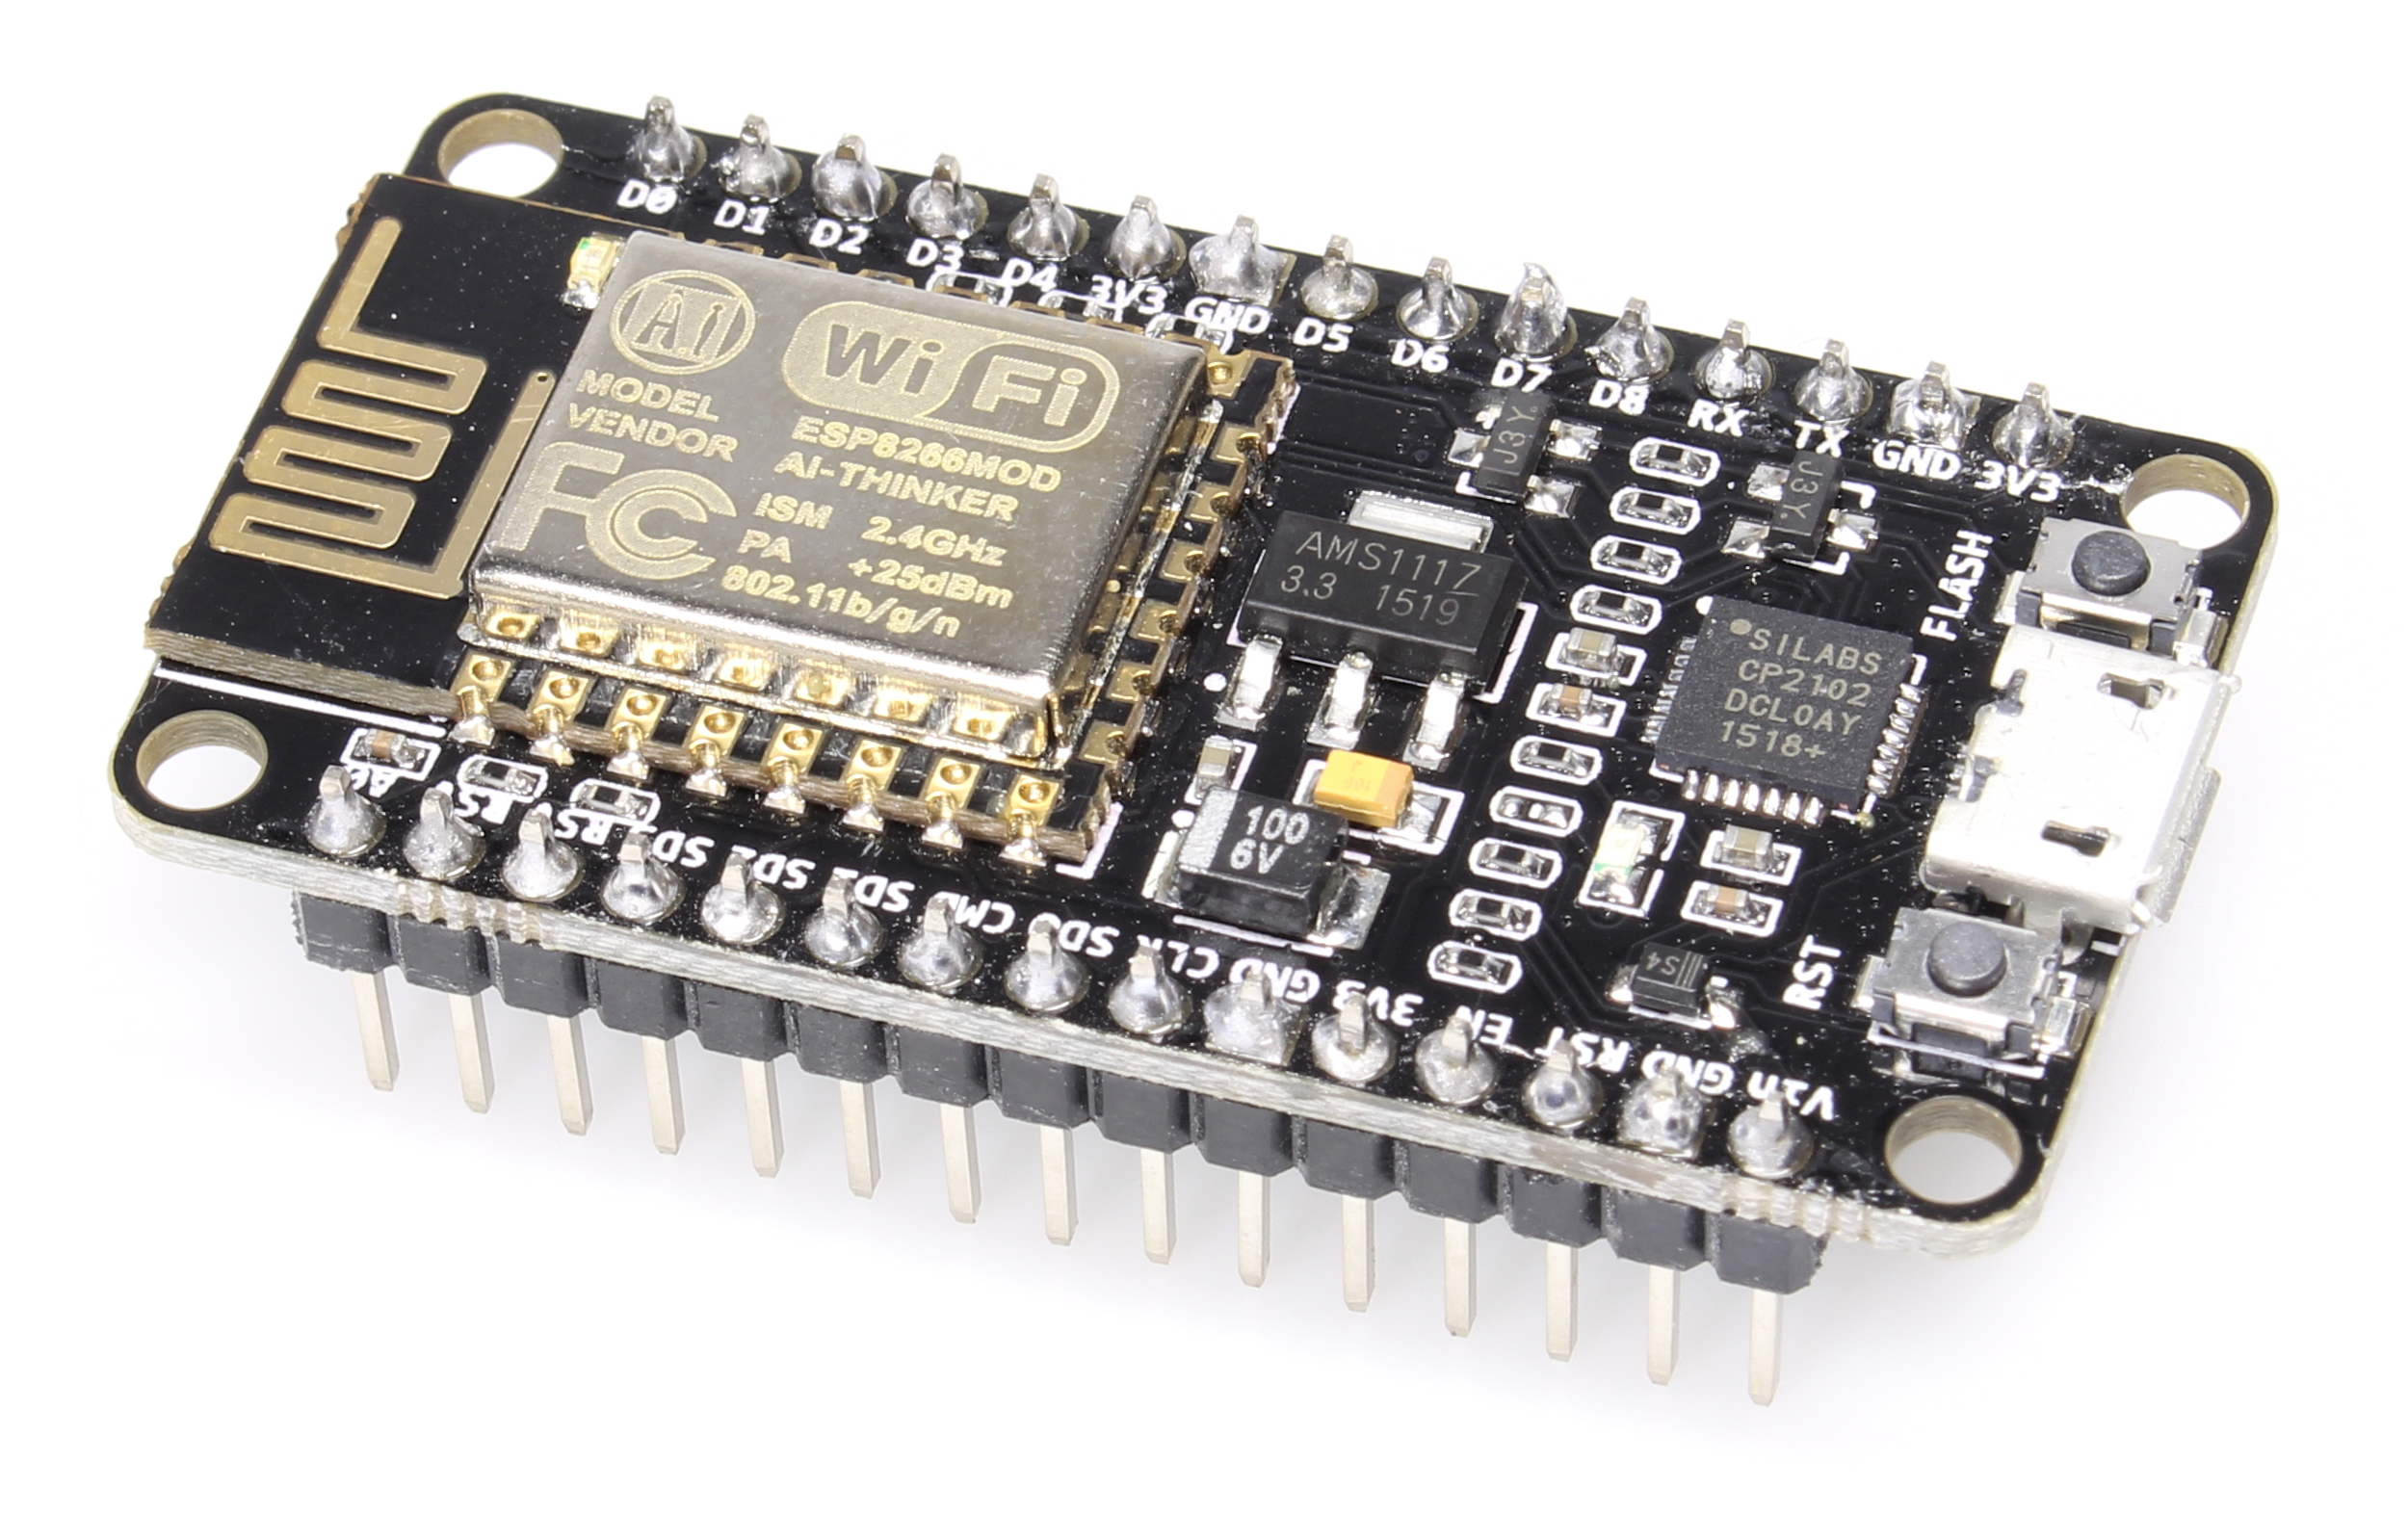
\includegraphics[scale=0.06]{imagens/nodemcu.png}
\caption{NodeMCU}
    \label{fig:nodemcu}
    \legend{FONTE: Autor}
\end{figure}

O NodeMCU é uma placa de desenvolvimento com módulo Wi-Fi integrado, compatível com as linguagens de programação: Lua, Python, 
JavaScript e IDE do Arduino.


\subsection{VL53L0X (Time-of-Flight)}

\begin{figure}[H]
\centering
\includegraphics[scale=0.1]{imagens/gy-vl53l0x.jpg}
\caption{VL53L0X-V2. (Time-of-Flight)}
    \label{fig:gy-vl53l0x}
    \legend{FONTE: Autor}
\end{figure}

O VL53L0X-V2 é um sensor a laser de tempo de vôo, ele é responsável por detectar quando o mosquito entra na armadilha e mandar as 
informações para o NodeMCU.

\section{Software}

Para receber e armazenar os dados provenientes das armadilhas foi desenvolvido uma API em NodeJS, utilizando o framework Express
e banco de dados Postgres.

\begin{figure}[H]
\centering
\includegraphics[scale=0.6]{imagens/diagramacloud.png}
\caption{Diagrama de infraestrutura}
    \label{fig:cloud}
    \legend{FONTE: Autor}
\end{figure}


O diagrama acima mostra a infraestrutura do projeto na nuvem, que foi hospedado utilizando os serviço do AWS da Amazon. O front-end está hospedado
utilizando o serviço de hospedagem de site estático Amazon S3. A API bem como o banco de dados estão rodando em containers Docker dentro de 
uma instância do Amazon EC2. A comunicação entre a aplicação cliente e a API é feita utilizando o protocolo HTTP e Web Socket.

\subsection{Banco de dados}

Para a tarefa de armazenar os dados provenientes das armadilhas das empresas/prefeituras e dos usuários da plataforma, 
foi escolhido o banco relacional Postgres. A figura abaixo mostra o diagrama de tabelas do banco:

\begin{figure}[H]
\centering
\includegraphics[scale=0.5]{imagens/EsquemaBanco.png}
\caption{Diagrama do banco}
    \label{fig:banco}
    \legend{FONTE: Autor}
\end{figure}

É inserido um novo registro na tabela ovitrap\_catches a cada captura feita por qualquer armadilha, isso possibilita gerar um gráfico do 
número de capturas em função do tempo.

As tabelas permission, profiles e profile\_permissions são responsáveis por fazer o controle de permissões do usuário na plataforma, 
uma vez que cada usuário tem um perfil e cada perfil possui permissões específicas para este. 

A tabela blacklists guarda os tokens
inválidos que são inseridos quando o usuário faz o logout ou quando seu token expira.

Para criação das tabelas e inserção dos perfis e permissões, foi escolhido o ORM Sequelize que gera a tabela SequelizeMeta para guardar as migrations
 que já foram executadas no banco.

\subsection{API}

A API para consumo dos dados armazenados no banco foi feita em NodeJS utilizando o framework Express. Todas as rotas (exceto login e 
esqueci minha senha) são protegidas por token, com 8h de duração. Todas as rotas contam com validação dos campos recebidos. 

Além de uma porta destinada a requisições HTTP, há outra porta destinada a comunicação via web socket, utilizando Socket.io, isso possibilita que a aplicação cliente 
receba dados em tempo real, como por exemplo, se houver uma captura de mosquito e o usuário estiver logado na plataforma o seu dashboard irá atualizar
no mesmo instante.

\subsection{Aplicação Cliente}

Para exibição dos dados em qualquer navegador web, a aplicação cliente foi desenvolvida utilizando ReactJS, redux-saga e MUI. A aplicação é responsiva e
conta com dois temas, claro e escuro, dois idiomas, português e inglês. 

\begin{figure}[H]
\centering
\includegraphics[scale=0.20]{imagens/front_1.png}
\caption{Tema claro}
    \label{fig:light}
    \legend{FONTE: Autor}
\end{figure}

\begin{figure}[H]
    \centering
    \includegraphics[scale=0.20]{imagens/front_2.png}
    \caption{Tema escuro}
        \label{fig:dark}
        \legend{FONTE: Autor}
    \end{figure}

No dashboard e no cadastro de armadilhas foram utilizados o serviço do Google Maps,
para exibição das armadilhas conforme sua latitude e longitude. No mapa, ao clicar em cada armadilha, é mostrado a 
quantidade total de mosquitos capturados pela armadilha.
Quando há uma captura em tempo real é mostrado o ícone de um mosquito acima da armadilha que realizou a captura.

\begin{figure}[H]
    \centering
    \includegraphics[scale=0.5]{imagens/front_5.png}
    \caption{Tela de login}
        \label{fig:login}
        \legend{FONTE: Autor}
    \end{figure}

Para o envio de emails para o usuário no cadastro e no reset de senha foi utilizado o serviço de envio de emails SendGrid.


\begin{figure}[H]
    \centering
    \includegraphics[scale=0.20]{imagens/front_4.png}
    \caption{Tela de listagem de armadilhas}
        \label{fig:listagem}
        \legend{FONTE: Autor}
    \end{figure}

A plataforma permite cadastrar, listar, alterar e deletar: empresas, usuários e armadilhas. 
Existem 3 perfis de usuários: Administradores do Sistema, Gestores e Agentes. 
Administradores do Sistema têm acesso a todas as funcionalidades do sistema.
Gestores têm acesso a todas as funcionalidades do sistema (exceto cadastrar, ler, alterar e deletar empresas/prefeituras).
Agentes somente podem ver as armadilhas da sua própria empresa, cadastrar novas armadilhas, alterar e deletar apenas
suas próprias armadilhas.

\begin{figure}[H]
    \centering
    \includegraphics[scale=0.20]{imagens/front_3.png}
    \caption{Tela de cadastro de armadilhas}
        \label{fig:cadastro}
        \legend{FONTE: Autor}
    \end{figure}


\section{Visão geral do sistema}

Juntando protótipo, sistema embarcado e sistema hospedado em nuvem, temos o seguinte diagrama:

\begin{figure}[H]
    \centering
    \includegraphics[scale=0.6]{imagens/diagramacloudarmadilha.png}
    \caption{Tela de cadastro de armadilhas}
        \label{fig:diagramacloudarmadilha}
        \legend{FONTE: Autor}
    \end{figure}


Nele temos uma visão completa do funcionamento do sistema, tudo começa no sensor da armadilha, que ao medir uma distância menor
que o range configurado faz uma chamada HTTP POST para API. A API por sua vez insere a nova captura na tabela de capturas, e 
envia um payload via socket para todos os usuários daquela empresa conectados. A aplicação recebe o payload e exibe uma nova captura
no mapa, no gráfico e na tabela.

\begin{figure}[H]
    \centering
    \includegraphics[scale=0.09, angle=-90]{imagens/IMG_0609.jpg}
    \caption{Protótipo final da armadilha em funcionamento}
        \label{fig:protótipofinal}
        \legend{FONTE: Autor}
    \end{figure}

\section{Custos}

Para construção do protótipo foram utilizados materiais que podem ser adquiridos facilmente na internet, lojas de materiais domésticos ou agrícolas.
Abaixo temos a tabela completa de todos os materiais e valores, cotados na data de publicação deste trabalho, na moeda brasileira real.

\begin{center}     
        \begin{table}[H]
            \caption{Tabela de custo}
            \label{tab:custos} 
            \begin{adjustbox}{width=\textwidth}  
        \begin{tabular}{ |c|c|c|c|c|c|c| }                           
            \hline
            \rowcolor{lightgray} \textbf{Descrição} & \textbf{Quantidade por lote} & \textbf{Unidade de medida} & \textbf{Valor lote} & \textbf{Valor por unidade} & \textbf{Quantidade utilizada} & \textbf{Valor total} \\
            \hline
            Vaso maior & 1 & un & 8,99 & 8,99 & 1 & 8,99 \\
            \hline
            Vaso menor & 1 & un & 1,99 & 1,99 & 1 & 1,99 \\
            \hline
            Boleira & 1 & un & 9,99 & 9,99 & 1 & 9,99 \\
            \hline
            Prato & 1 & un & 1,99 & 1,99 & 1 & 1, \\
            \hline
            Tela com velcro & 1,95 & $m^{2}$ & 12,99 & 6,66 & 0,066 & 0,44 \\
            \hline
            Breu & 100 & g & 7,7 & 0,08 & 100 & 7,70 \\
            \hline
            Palito Churrasco & 100 & un & 15 & 0,15 & 2 & 0,30 \\
            \hline
            Fita herllerman 120mm & 100 & un & 4,99 & 0,05 & 3 & 0,15 \\
            \hline
            Bastao cola quente & 10 & un & 5,99 & 0,60 & 1 & 0,60 \\
            \hline
            Jumpers & 120 & un & 20,72 & 0,17 & 54 & 9,32 \\
            \hline
            Protoboard & 1 & un & 15 & 15,00 & 1 & 15,00 \\
            \hline
            NodeMCU & 1 & un & 25,5 & 25,50 & 1 & 25,50 \\
            \hline
            Vl53X-V2 & 1 & un & 13,79 & 13,79 & 5 & 68,95 \\
            \hline
            Cabo micro USB & 1 & un & 4,9 & 4,90 & 1 & 4,90 \\
            \hline
            Fonte de tomada USB 5v & 1 & un & 10,23 & 10,23 & 1 & 10,23 \\
            \hline           
            &  &  &  &  & \textbf{Total} & \textbf{166,05} \\
            \hline
        \end{tabular}  
    \end{adjustbox}
    \end{table}    
\end{center}

Observamos a partir da tabela acima que o custo com componentes eletrônicos foi de R\$133,904 que representa 80,64\% do valor total do protótipo e que o custo com 
componentes estruturais foi de R\$32,15 que representa 19,36\% do valor total do protótipo.

\chapter{Conclusão e trabalhos futuros}

Baseado nos testes realizados com o protótipo em campo aberto, observou-se que a maior dificuldade é atrair mosquitos para armadilha, sendo que esta foi deixada por uma semana em
no jardim, e não foi capturado nenhum mosquito. Houve alguns registros do  sensor, porém nenhum mosquito foi capturado pela cola interna da armadilha. A cola desenvolvida com breu,
após alguns dias derreteu e caiu na tela mosquiteira da armadilha devido ao calor do sol. Após alguns meses a cola ressecou e perdeu sua aderência. Apesar do protótipo
não ter sucesso em capturar mosquitos, todo o restante da aplicação se saiu bem, em testes com objetos maiores ou com chamadas HTTP que simulam uma armadilha real. A plataforma está 
consistentes e pode ser replicada para qualquer outra rede de sensores com pouquíssimas modificações, a estrutura do banco está bem definida e todo o sistema de perfis e 
permissões podem ser customizados de acordo com a necessidade do cliente.

Como trabalhos futuros temos os seguintes itens: 

\begin{itemize}
    \item Nível de protótipo
    \begin{itemize}
        \item Validar o protótipo da armadilha, em ambiente controlado e em ambiente aberto. Analisar e comparar os resultados e a eficácia da mesma.
        \item Analisar o uso de substâncias com cheiro atrativo para o mosquito, como por exemplo, a alfafa prensada.
        \item Analisar a viabilidade de se trocar o sensor laser por um sensor sonoro, com aplicação de filtro para a frequência sonora de vôo do mosquito.
        \item Procurar alternativas melhores para cola no interior da armadilha como: fitas prega-rato ou fitas prega-mosca e/ou incluir uma 
        ventoinha abaixo da abertura, para que o mosquito seja sugado para dentro da armadilha.
    \end{itemize}
    \item Nível de aplicação
    \begin{itemize}
        \item Cadastrar o id da armadilha, nome e senha da rede wifi de maneira dinâmica.
        \item Melhorar a aplicação para que seja possível cadastrar uma foto de perfil para o usuário.
    \end{itemize}   
\end{itemize}


% ----------------------------------------------------------
% Referências bibliográficas
% ----------------------------------------------------------

\chapter*{REFERÊNCIAS}
\addcontentsline{toc}{chapter}{REFERÊNCIAS}
\renewcommand{\bibsection}{}
\bibliography{bibliografia.bib}


% ----------------------------------------------------------
% ELEMENTOS PÓS-TEXTUAIS
% ----------------------------------------------------------
\chapter*{APENDICE A - DOCUMENTO DE REQUISITOS}
\addcontentsline{toc}{chapter}{APENDICE A - DOCUMENTO DE REQUISITOS}

\input{docreq}

% ----------------------------------------------------------


%---------------------------------------------------------------------

% INDICE REMISSIVO
%---------------------------------------------------------------------
\phantompart
\printindex

%---------------------------------------------------------------------
\end{document}

